\documentclass{beamer}
\usetheme{Madrid}
\usepackage{subcaption}
\usepackage{tikz}
\usetikzlibrary{positioning} 
\usetikzlibrary{matrix}
\usetikzlibrary{calc}
\newcommand{\z}{\mathbf{z}}
\newcommand{\uout}{u_{out}}
\newcommand{\vout}{v_{out}}
\newcommand{\uoutdum}{u_{out}^{dum}}
\newcommand{\uinplus}{u_{in}^{+}}
\newcommand{\uinminus}{u_{in}^{-}}
\newcommand{\winl}{w_{in}^{l}}
\newcommand{\win}{w_{in}}
\newcommand{\uin}{w_{in}}
\newcommand{\vin}{v_{in}}

\DeclareMathOperator*{\plusrightarrow}{\ensuremath{\xrightarrow{+}}}
\DeclareMathOperator*{\minusrightarrow}{\ensuremath{\xrightarrow{-}}}
\DeclareMathOperator*{\plusleftarrow}{\ensuremath{\xleftarrow{+}}}
\DeclareMathOperator*{\minusleftarrow}{\ensuremath{\xleftarrow{-}}}
\usetikzlibrary{shadows,positioning}
\colorlet{colD}{red!40}
\colorlet{colIP}{cyan!40}
\colorlet{colV}{blue!40}
\colorlet{colBorder}{gray!70}


\title[Singed Network Embeddings]{ROSE: Role-based Signed Network Embedding
}

\author[Javari et al.]{Amin Javari \and Tyler Derr \and Pouya Esmailian \and Jiliang Tang \and Kevin Chen-Chuan Chang}
\date{\today}

\begin{document}
\begin{frame}
    \titlepage
\end{frame}

\begin{frame}
    \frametitle{Overview}
    \tableofcontents
\end{frame}


\section{Motivation}
\begin{frame}
    \frametitle{Motivation}

    \begin{itemize}
        
        \item Graphs are universal data structures (maybe quite literally? \cite{wolfram2020class})
        \item But
        \begin{enumerate}
            \item Have a large computational complexity for storage as well as usage
            \item Low parallelizability
            \item Supervised Machine Learning tasks require handcrafted features for each graph
        \end{enumerate}
        \item We wish to learn dense, continuous and low dimensional representation  for nodes \cite{Cui_2019Survey}
        \item Use these Embeddings to solve many downstream tasks
        \begin{itemize}
            \item Node importances
            \item Community Detection
            \item Link Prediction
            \item Node classification
        \end{itemize}
    \end{itemize}

\end{frame}

\section{Network Embedding Survey}
\begin{frame}
    \frametitle{Survey of existing techiques}

    \begin{itemize}
        \item A high level view of the existing Network Embedding approaches \cite{chami2020machine}
        \item Graph Encoder Decoder Model (GraphEDM) as a framework 
        \item Graph $G=(V,R)$, weight matrix $W\in \mathbb{R}^{|V|\times|V|}$
        \item Optional \textit{node features} of dimension $d_{0}$, $X \in \mathbb{R}^{|V|\times d_{0}}$
        \item Goal is to learn a vector representation, $Z \in \mathbb{R}^{|V|\times d}$, where $d \ll |V|$
    \end{itemize}
    
\end{frame}
\begin{frame}
    \frametitle{GraphEDM Framework and Objective Functions}
    \begin{figure}[htp]
        \centering
        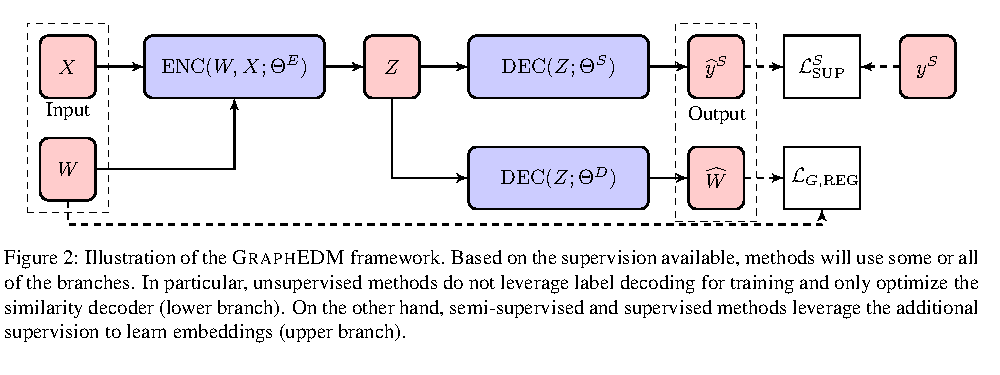
\includegraphics[width=0.5\textwidth]{images/graphEDM-crop.pdf}
    \end{figure}
    \begin{enumerate}
        \item Supervised Loss $\mathcal{L}_{SUP}^{S}$
        \begin{itemize}
            \item Compares predicted labels $\widehat{y}^{S}$ to ground truth $y^{S}$
        \end{itemize}
        \item Graph Regularization loss $\mathcal{L}_{G,REG}$
            \begin{itemize}
                \item Regularizes model parameters based on graph structure 
                \item $\mathcal{L}_{G,REG}(W,\widehat{W};\theta) =d_{1}(s(W),\widehat{W})$
                \item $s(W)$ is target similarity matrix and $d_{1}(\cdot,\cdot)$ distance function
            \end{itemize}
        \item Weight Regularization loss $\mathcal{L}_{REG}$
            \begin{itemize}
                \item Used as prior, most common Gaussian prior (L2 regularization)
                \item $\mathcal{L}_{\mathrm{REG}}(\Theta)=\sum_{\theta \in \Theta}\|\theta\|_{2}^{2}$
            \end{itemize}
    \end{enumerate}
    \begin{block}{GraphEDM Total Loss}
        $\mathcal{L}=\alpha \mathcal{L}_{\mathrm{SUP}}^{S}\left(y^{S}, \hat{y}^{S} ; \Theta\right)+\beta \mathcal{L}_{G, \mathrm{REG}}(W, \widehat{W} ; \Theta)+\gamma \mathcal{L}_{\mathrm{REG}}(\Theta)$
        \end{block}

\end{frame}
\begin{frame}
    \frametitle{}
    \label{slide:taxonomy}
    \begin{figure}[htp]
        \centering
        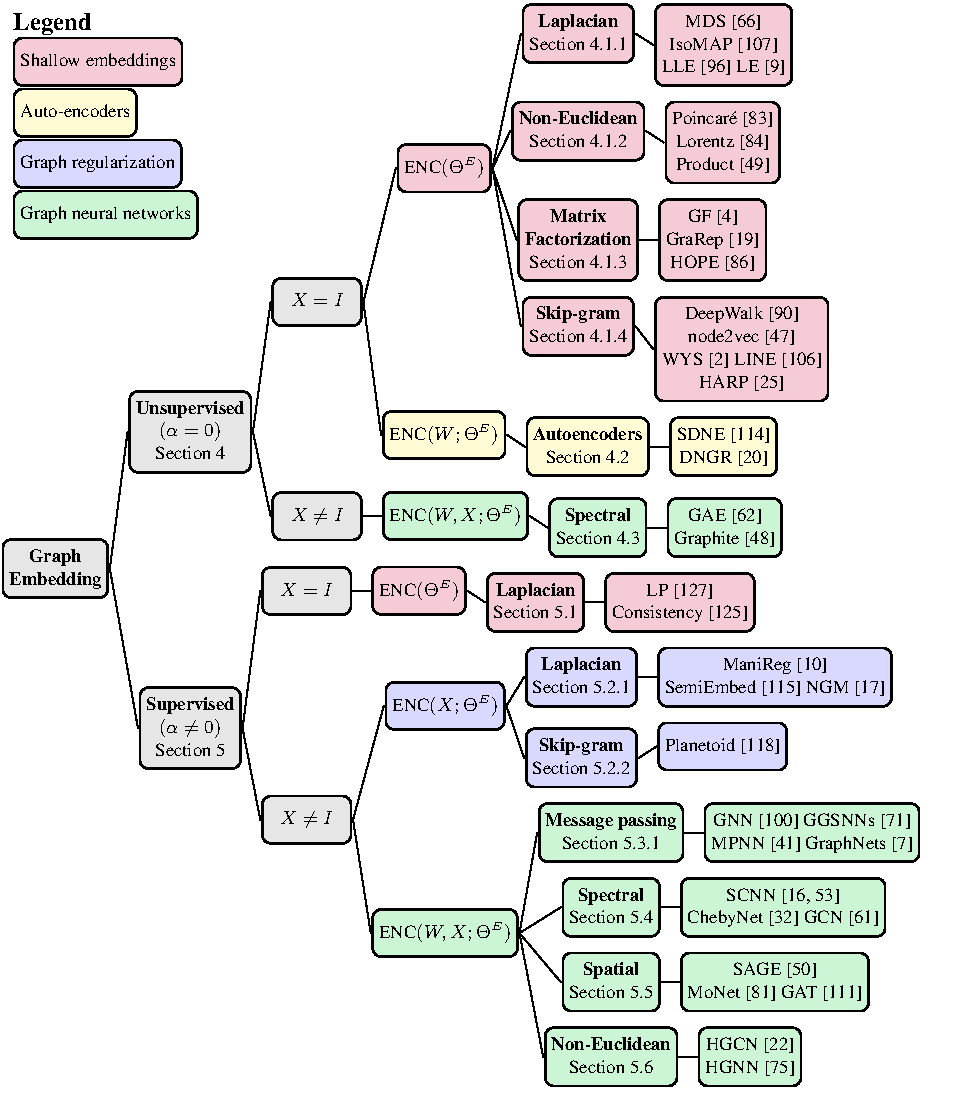
\includegraphics[width=0.5\textwidth]{images/taxonomy-crop.pdf}
        \caption{Taxonomy Proposed by \cite{chami2020machine}}
    \end{figure}

\end{frame}

\subsection{Skip-Gram Based Embeddings}

\begin{frame}
    \frametitle{Shallow Encodings}
    \begin{itemize}
        \item $Z = ENC(\Theta^{E}) = \Theta^{E} \in \mathbb{R}^{|V|\times d}$
        \item Each node $v \in V$ has a unique encoding vector $\mathbf{z}_{v}$ 
        \item Just a simple embedding lookup
        \item Similarity between nodes $u$ and $v$ in embedding space is dot product $\mathbf{z}_{u}^{\top}\mathbf{z}_{v} $
        \item What the similarity will be in the original network?
        \begin{itemize}
            \item Adjacency
            \item Shared Neighbours
            \item Structural Roles
        \end{itemize}
    \end{itemize}
\end{frame}

\begin{frame}
    \frametitle{Random Walk Embeddings}
    \begin{itemize}
        \item Use a random walk strategy $R$ to estimate probability of visiting $v$ when starting from $u$, $P_{R}(v\mid u)$
        \item Train embeddings such that for every pair $\mathbf{z}_{u}^{\top}\mathbf{z}_{v} \propto P_{R}(v\mid u)$
        \item Why Random Walks?
        \begin{itemize}
            \item Incorporate local and global network information
            \item Highly efficient to generate random Walks
            \item Unsupervised approach
        \end{itemize}
        \item E.g, DeepWalk \cite{Perozzi_2014} and node2vec \cite{Grover_2016}
    \end{itemize}
\end{frame}


\begin{frame}
    \frametitle{Learn Random Walk Embeddings}
    \begin{itemize}
        \item Use \textit{skip-grams} theory from language model literature \cite{mikolov2013distributed}
        \item Neighbourhood $N_{R}(u)$ for a node $u$ from the random walk strategy $R$  
        \item Minimize the following loss function $\mathcal{L}$ using SGD
    \end{itemize}
    \[ \mathcal{L} = \sum_{u\in V}\sum_{v \in N_{R}(u)} -\log\left( P(v\mid \mathbf{z}_{u}) \right),  \]
    \begin{itemize}
        \item Define the probability as a softmax
    \end{itemize}
    \[P(v \mid \mathbf{z}) = \frac{\exp(\mathbf{z}_{u}^{\top}\mathbf{z}_{v})}{\sum_{n \in V}\mathbf{z}_{u}^{\top}\mathbf{z}_{n}} \]
    \begin{itemize}
        \item Drawback is that $\mathcal{L}$ has a quadratic complexity $\mathcal{O}(|V|^{2})$
    \end{itemize}
\end{frame}

\begin{frame}
    \frametitle{Fix Softmax}
    Again language model literature has two proposed solutions \cite{mikolov2013distributed}
        \begin{enumerate}
            \item Hierarchical Softmax
            \begin{itemize}
                \item Reduced complexity of computing $P(v \mid \mathbf{z}_{k})$ from $\mathcal{O}(|V|)$ to $\mathcal{O}(\log|V|)$
                \item Can be further optimized using Huffman encoding etc.
                \item E.g. DeepWalk \cite{Perozzi_2014}
            \end{itemize}
            \item Negative Sampling 
            \begin{itemize}
                \item Approximate using negative samples $n_{i} \sim P_{V}$ and sigmoid function $\sigma(x) = 1/(1+e^{-x})$ 
                \[ \log(P(v\mid \mathbf{z}_{u}))\approx\log\left(\sigma\left(\mathbf{z}_{u}^{\top} \mathbf{z}_{v}\right)\right)-\sum_{i=1}^{k} \log \left(\sigma\left(\mathbf{z}_{u}^{\top} \mathbf{z}_{n_{i}}\right)\right)\]
                \item Sample $k$ negative nodes proportional to the degree
                \item Empirically better than hierarchical softmax
                \item E.g., node2vec \cite{Grover_2016}
            \end{itemize}
        \end{enumerate}
\end{frame}

\begin{frame}
    \frametitle{How to Walk?}
    \begin{enumerate}
        \item Unbiased Random Walks \cite{Perozzi_2014}
        \item Biased Random Walks \cite{Grover_2016}
        \begin{itemize}
            \item Allows to tune between \textit{local} (BFS) and \textit{global} (DFS) walks
            \item Add return probability  $p$ and walk-away probability $q$ to random walks
            \item Low $p$ similar to BFS abd low $q$ similar to DFS
        \end{itemize}
        \begin{figure}[htp]
            \centering
            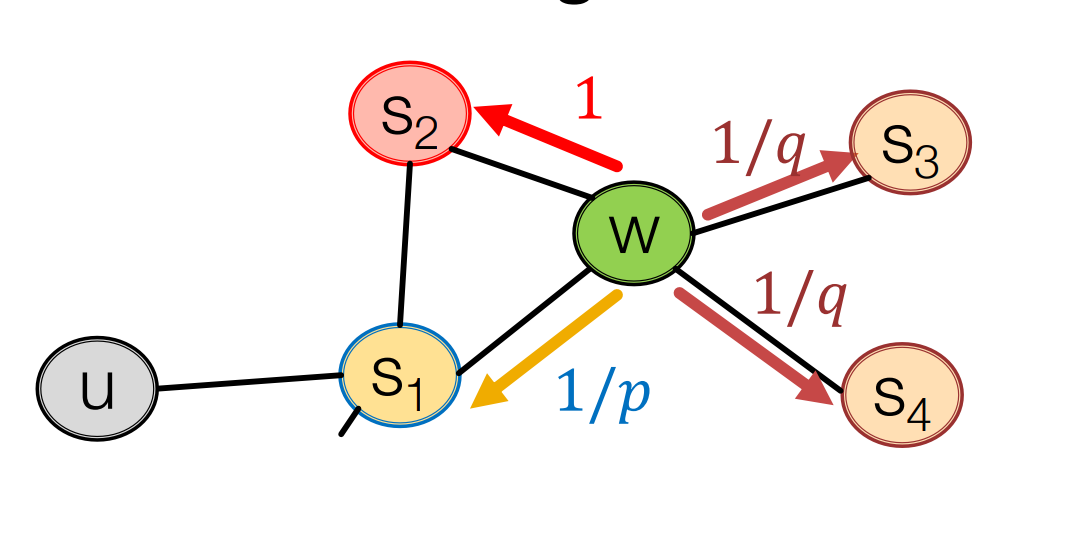
\includegraphics[width=0.5\textwidth]{images/biased-walk.png}
            \caption{From lecture slides \cite{Leskovec2018cs224w}}
        \end{figure}
    \end{enumerate}
    
\end{frame}

\begin{frame}
    \frametitle{node2vec Algorithm}
    \begin{enumerate}
        \item Choose probabilities $p$ and $q$ and compute random walk probabilities 
        \item Generate $r$ random walks of length $l$ from each starting node
        \item Learn embeddings by optimizing loss with SGD or directly use \texttt{gensim} word2vec trainer
    \end{enumerate}
    

\end{frame}
\subsection{Signed Network Embeddings}

\begin{frame}
    \frametitle{Additional Hurdles in Signed Grpahs}
    \begin{itemize}
        \item Conventional unsigned embedding techniques misunderstand signed edges
        \item Traditional negative sampling does not work as expected
        \item Incorporate structural theories of \textit{Balance} and \textit{Status}?
        \item Considering cycles and long path features
        \item Learn asymmetric embeddings for directed graphs
    \end{itemize}

\end{frame}

\begin{frame}
    \frametitle{Existing Approaches}
    \begin{enumerate}
        \item \textbf{SiNE} (Signed Network Embeddings) \cite{Wang2017SiNE}
        \begin{itemize}
            \item<2-> Multilayer Neuaral Network
            \item<2-> Optimizes objective function that satisfies balance theory
            \item<2-> Only for undirected graphs
        \end{itemize}
        \item \textbf{SIDE} (SIgned Directed network Embedding) \cite{Kim2018_SIDE}
        \begin{itemize}
            \item<3-> Random Walk based approach
            \item<3-> Aggregates sign of co-occurring nodes in a walk using balance theory
            \item<3-> Accordingly changes likelihood for loss term
            \item<3-> Works for directed and undirected networks
        \end{itemize}
        \item \textbf{SIGNet} (SIGned Network embeddings) \cite{Islam_2018_sign2vec}
        \begin{itemize}
            \item<4-> Also random walk based
            \item<4-> Uses targeted negative sampling along with balance theory
        \end{itemize}
        \item \textbf{BESIDE} (Bridge Enhanced Signed Directed Network Embedding) \cite{Chen2018_BESIDE}
        \begin{itemize}
            \item<5-> Utilizes bridge edges to encode status theory based features
            \item<5-> Uses triads to encode balance theory based features
            \item<5-> Creates a combined loss function and optimizes using mini-batch SGD
        \end{itemize}
    \end{enumerate}
\end{frame}


\section{ROSE}

\begin{frame}
    \frametitle{ROSE: Role-based Signed Network Embedding
    }

    What they aim to Fix
    \begin{enumerate}
        \item A general framework not based on social theories
        \begin{itemize}
            \item Social theories of balance and status are restrictive 
            \item They might be inaccurate in certain networks
            \item May not consider longer cycle features when creating embeddings
        \end{itemize}
        \item Utilize missing links as information
        \begin{itemize}
            \item Most models utilize negative and positive links 
            \item Cannot predict the absence of links between nodes 
        \end{itemize}
    \end{enumerate}
\end{frame}

\begin{frame}
    \frametitle{ROSE: Role-based Signed Network Embedding}
    What they propose 
    \begin{itemize}
        \item Network transformation based embedding
        \item Convert signed network to a unsigned bipartite network
        \item Model each original node using several "role" nodes
        \item Embed the transformed network using traditional methods
        \item Aggregate the "role" node embeddings to get original node embeddings
    \end{itemize}
\end{frame}

\subsection{Network Transformation}
\begin{frame}
    \frametitle{Network Transformation}
    \begin{enumerate}
        \item<1-> Transform to Bipartite Network
        \begin{itemize}
            \item<2-> Each node has a "\textit{user}" role for out edges and "\textit{item}" role for in edges
            \item<2-> Split each node $u$ into $u_{out}$ and $u_{in}$ and map edges 
            \item<2-> Still has signed edges
        \end{itemize}
        \item<1-> Transform to Unsigned Bipartite Network
        \begin{itemize}
            \item<3-> Split each role $u_{in}$ further into $u_{in}^{+}$ and $u_{in}^{-}$
            \item<3-> Remap signed edges as unsigned edges to positive and negative role nodes respectively
            \item<3-> Can now use traditional similarity measures
        \end{itemize}
        \item<1-> Augment Network
        \begin{itemize}
            \item<4-> Negative links are under-represented in signed networks
            \item<4-> Roles of $in^{-}$ has very low degree
            \item<4-> Assume $u_{out}$ is connected to $v_{in}^{+}$ and $w_{in}^{-}$
            \item<4-> This implies $v_{in}^{+}$ and $w_{in}^{-}$  are adjacent \textbf{and also} $v_{in}^{-}$ and $w_{in}^{+}$ are related  
            \item<4-> Add dummy $u_{out}^{dum}$ and connect opposite role nodes
        \end{itemize}
    \end{enumerate}
    
    \uncover<5->{Let's see an example}

\end{frame}

\begin{frame}
    \frametitle{Network Transformation Example}
    \tikzset{
  invisible/.style={opacity=0},
  visible on/.style={alt={#1{}{invisible}}},
  alt/.code args={<#1>#2#3}{%
    \alt<#1>{\pgfkeysalso{#2}}{\pgfkeysalso{#3}} % \pgfkeysalso doesn't change the path
  },
  position/.style args={#1:#2 from #3}{
        at=(#3.#1), anchor=#1+180, shift=(#1:#2)
    },
}


\begin{tikzpicture}
    \begin{scope}[
        every node/.style={draw,circle,thick,scale=0.5,minimum size=1.2cm}
        ]
        \node (1) at (0,0) {$1$};
        \node[position=-120:1cm from 1] (2) {$2$};
        \node[position=-60:1cm from 1] (3) {$3$};

        \node[below left=1.5cm and 4cm of 2] (1out) {$1_{out}$};
        \node[right=0.5cm of 1out] (2out) {$2_{out}$};
        \node[right=0.5cm of 2out] (3out) {$3_{out}$};
        \node[below=1cm of 1out] (1in) {$1_{in}$};
        \node[below=1cm of 2out] (2in) {$2_{in}$};
        \node[below=1cm of 3out] (3in) {$3_{in}$};
        
        \node[right=4cm of 3out] (1out') {$1_{out}$};
        \node[right=0.5cm of 1out'] (2out') {$2_{out}$};
        \node[right=0.5cm of 2out'] (3out') {$3_{out}$};
        
        \node[right=2.5cm of 3in,green,text=black] (1in+) {$1_{in}^{+}$};
        \node[right=0.5cm of 1in+,red,text=black] (1in-) {$1_{in}^{-}$};
        \node[right=0.5cm of 1in-,green,text=black] (2in+) {$2_{in}^{+}$};
        \node[right=0.5cm of 2in+,red,text=black] (2in-) {$2_{in}^{-}$};
        \node[right=0.5cm of 2in-,green,text=black] (3in+) {$3_{in}^{+}$};
        \node[right=0.5cm of 3in+,red,text=black] (3in-) {$3_{in}^{-}$};
        
        \node[below=3cm of 1out',visible on =<14->] (1outd) {$1_{out}^{dum}$};
        \node[below=3cm of 2out',visible on =<14->] (2outd) {$2_{out}^{dum}$};
        \node[below=3cm of 3out',visible on =<14->] (3outd) {$3_{out}^{dum}$};
    \end{scope}
    
    \begin{scope}[
        positive/.style = {draw,thick,green,-latex,>=stealth},
        negative/.style = {draw,thick,red,-latex,>=stealth},
        positive'u/.style = {draw,thick,green},
        negative'u/.style = {draw,thick,red},
        normal/.style = {draw,thick},
        dummy/.style = {draw,thick,dashed},
        highlight/.style={draw,thick,yellow,-,double=yellow,double distance=4\pgflinewidth}
    ]
    \path 
    (1) edge[positive,bend right=40,preaction={highlight,visible on=<2-4>}] (2)
    (2) edge[negative,bend right=40,preaction={highlight,visible on =<5-7>}] (1)
    (2) edge[negative,preaction={highlight,visible on=<8-10>}] (3)
    (3) edge[positive,preaction={highlight,visible on=<11-13>}] (1)
    ; 
    \path
    (1out) edge[positive'u,visible on=<3->] (2in)
    (2out) edge[negative'u,visible on=<6->] (1in)
    (2out) edge[negative'u,visible on=<9->] (3in)
    (3out) edge[positive'u,visible on=<12->] (1in)
    ;
    
    \path
    (1out') edge[normal,visible on=<4->] (2in+)
    (2out') edge[normal,visible on=<7->] (1in-)
    (2out') edge[normal,visible on=<10->] (3in-)
    (3out') edge[normal,visible on=<13->] (1in+)
    ;
    
    \path
    (1outd) edge[dummy,visible on =<15->] (2in-)
    (2outd) edge[dummy,visible on =<15->] (1in+)
    (2outd) edge[dummy,visible on =<15->] (3in+)
    (3outd) edge[dummy,visible on =<15->] (1in-)
    ;
    \end{scope}

    \begin{scope}[
        every node/.style={draw=none,rectangle},
        every edge/.style={draw=none},
    ]
    \path 
    (2) edge node[above=1.5cm] {Signed Network} (3)
    (1out) edge node[above=0.5cm] {Bipartite Signed Network} (3out)
    (1out') edge node[above=0.5cm] {Unsigned Bipartite Role Network} (3out')
    ;
    \end{scope}
\end{tikzpicture}
\end{frame}

\begin{frame}
    \frametitle{Network Transformation Summary}
    \begin{itemize}
        \item Graph $G=(V,E)$ transformed to bipartite unsigned $G_{u}=(V_{u},E_{u})$
        \item $|V_{u}|=4|V|$ and $|E_{u}|=2|E|$
        \item Each $u \in V$ becomes $u_{out},u_{in}^{+},u_{in}^{-},u_{out}^{dum} \in V_{u}$
        \item Each $(u,v) \in E$ with label $l$ becomes $(u_{out},v_{in}^{l})$ and $(u_{out}^{dum},v_{in}^{l^{\prime}})$
        \item Transformation is \textbf{lossless}
    \end{itemize}

\end{frame}


\subsection{Embedding}
\begin{frame}
    \frametitle{Embedding the Network}
    \begin{itemize}
        \item After network transformation we have traditional network
        \item Can employ any classic embedding scheme (see Slide~\ref{slide:taxonomy})
        \item Paper uses well known node2vec
        \item Now each role node has an embedding, $\z_{\uout},\z_{\uinplus},\z_{\uinminus},\z_{\uoutdum}$
        \item Paper proposed two methods to get the embedding of $u$ of the original network
    \end{itemize}
\end{frame}

\begin{frame}
    \frametitle{Aggregation Strategies}
    \begin{enumerate}
        \item Fixed Aggregation
        \begin{itemize}
            \item Simplest approach to concatenate all representations
            \item $\z_{u} = [\z_{\uout},\z_{\uinplus},\z_{\uinplus}]$
            \item Dummy nodes are not used, $\z_{\uoutdum}$ is inverse of $\z_{\uout}$
        \end{itemize}
    \item Target Aware Aggregation
    \begin{itemize}
        \item Useful for tasks such as link prediction
        \item Analogous to item-based collaborative filtering: predict rating of users towards a particular item 
        \item Use a weighted combination based on similarity to target item
        \item Embed the "out" node $\uout$ wrt target node $v$, $\z_{\uout}^{v}$
        \item Combine target aware embedding along with personal embedding to get $u$ wrt $v$
    \end{itemize}
    \[ \z_{u}^{v} = [z_{\uout}^{v},\z_{u}].\]
    \end{enumerate}
\end{frame}

\begin{frame}
    \frametitle{Attention Embedding}
    \begin{itemize}
        \item Compute $\z_{\uout}^{v}$ as a weighted sum of the neighbours $\uout$
        \item Each neighbour $\winl \in N(\uout)$, where $l$ is either $+$ or $-$
    \end{itemize}
    \[\z_{\uout}^{v}  = \sum_{\winl \in N(\uout)} attn(\winl,v)\z_{\winl},\]
    \begin{itemize}
        \item Weight $attn(\winl,v)$ is how relevant that neighbour is towards the target node $v$
        \item Intuition is that "in" nodes are more related if closer in network
        \item Label is not considered, so need $\z_{\uin}$ for every node 
        \item Ignore signs of original network and convert to bipartite and get node2vec embeddings
    \end{itemize}    
    \[ attn(\winl,v) = \sigma(\z_{\win},\z_{\vin}) = \frac{1}{1+\exp(-\z_{\win}^{\top}\z_{\vin})} .
    \]
\end{frame}

\subsection{Results}

\begin{frame}
    \frametitle{Results}
    \label{slide:results}
     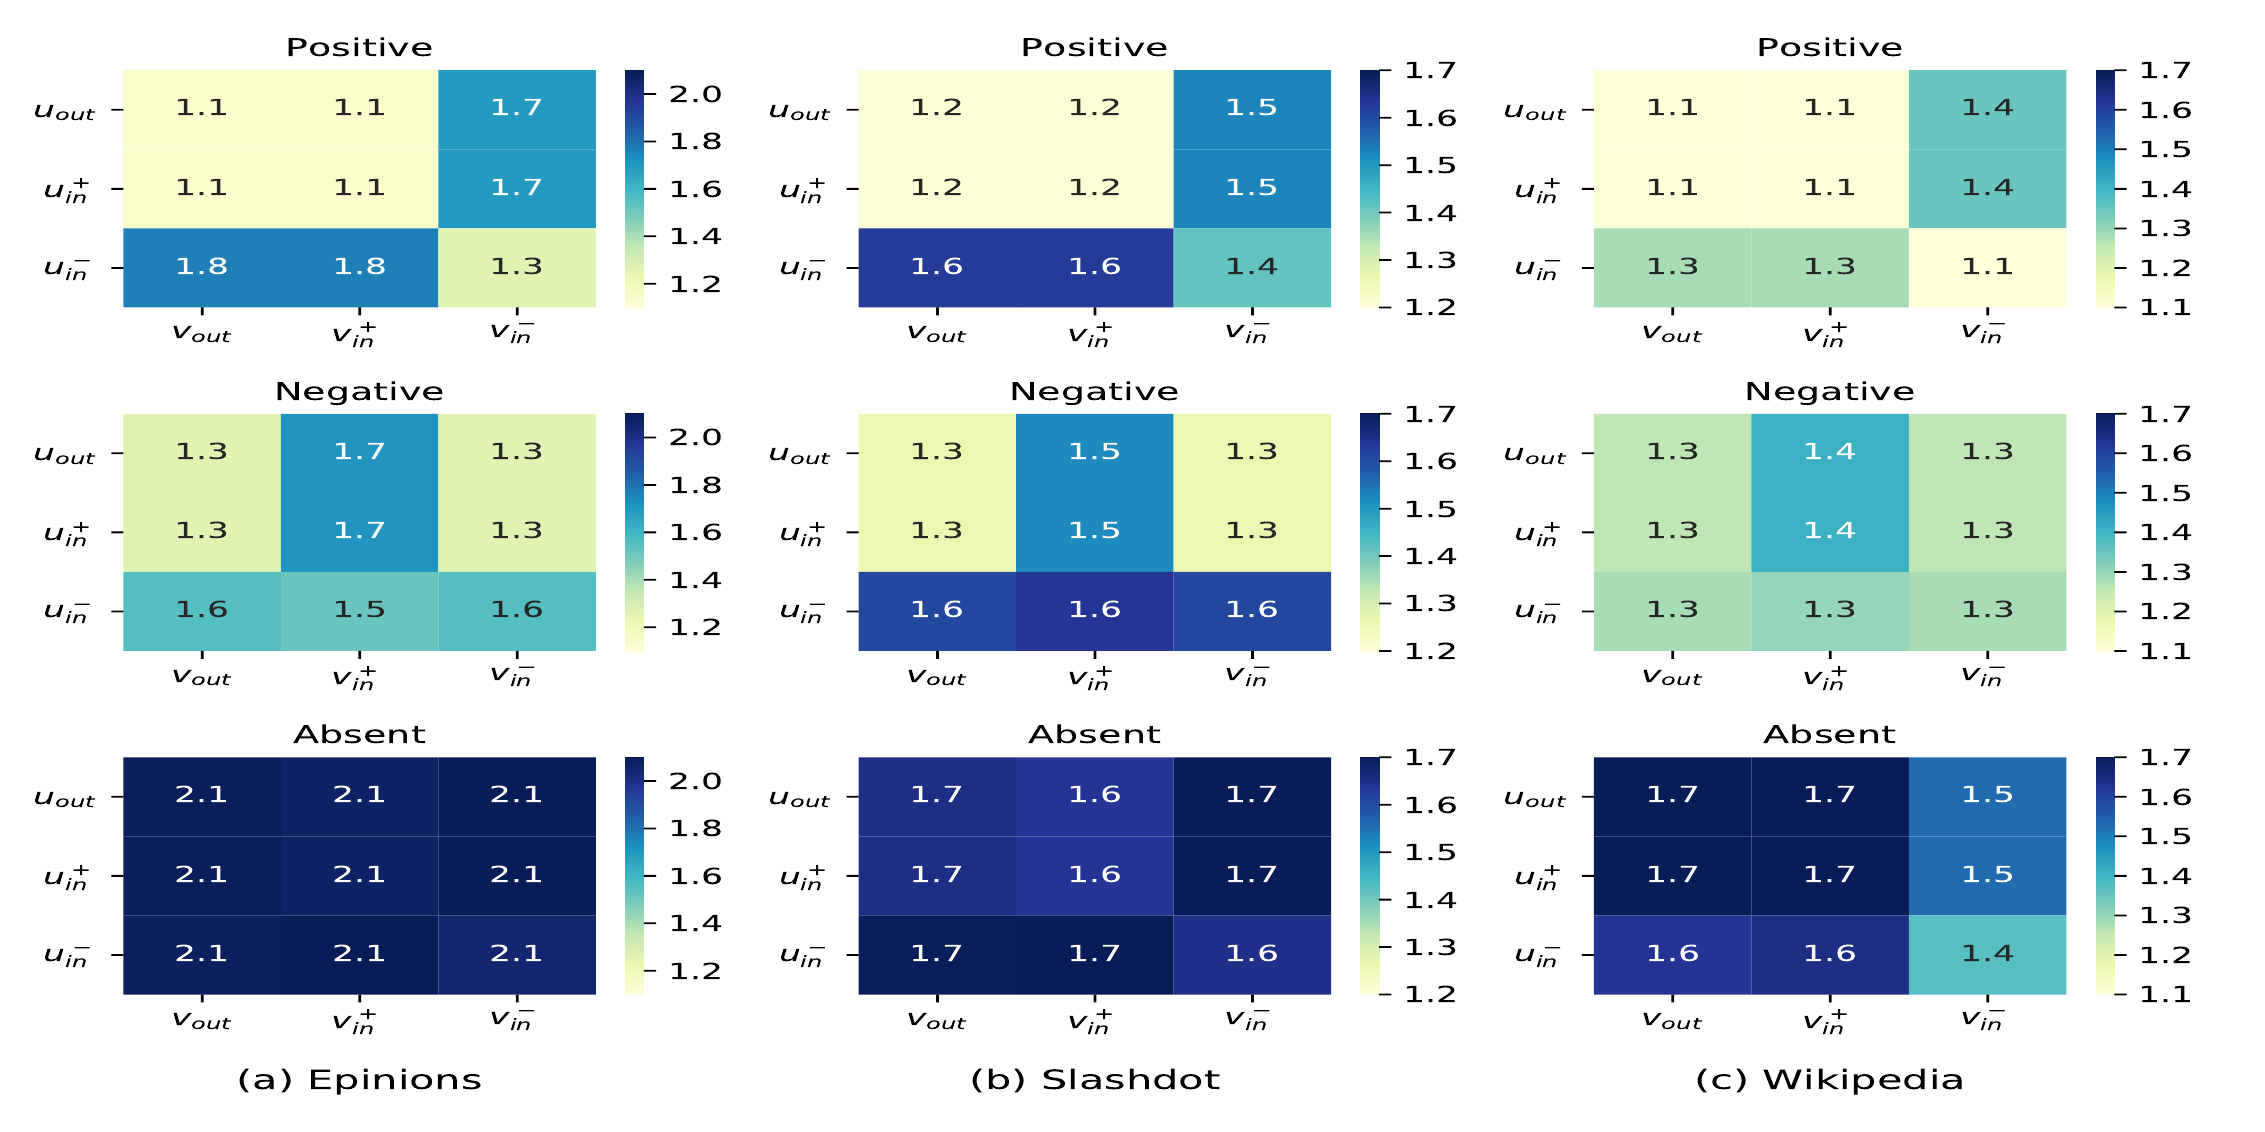
\includegraphics[width=\textwidth]{images/results.png}   

\end{frame}

 \begin{frame}
     \frametitle{Interpretations of Role Nodes}
    \begin{itemize}
        \item Label of link from $u$ to $v$ is $l$ if $\z_{\uout}$ is closer to $\z_{\vin^{l}}$ than $\z_{\vin^{l^\prime}}$
        \item If $\z_{\uout}$ is further apart from both $\z_{\vin^{+}}$ and $\z_{\vin^{-}}$, then the link is absent
        \item See $d_{avg}(\uout,\vin^{+})$ compared to $d_{avg}(\uout,\vin^{-})$
        \item $d_{avg}(\uout,\vin^{+})+d_{avg}(\uout,\vin^{-})$ is smaller when there is a link compared to when there is no link.
        \item There are \textbf{four} \textit{implicit patterns} apart from this
        \item They analyse situations for a pair of nodes $u$ and $v$ 
    \end{itemize}
\end{frame}

\begin{frame}
    \frametitle{Intersting Patterns}
    \begin{enumerate}
        \item \textit{Pattern 1}: Incoming Edges 
        \begin{itemize}
            \item "If the sign of the link from $u$ to $v$ is positive, similar nodes rate them similarly and if it is negative, similar nodes rate them with different signs"
            \item If edge $u \plusrightarrow v$, incoming edges are similar
            \item $d_{avg}(\uinplus,\vin^{+})$ and $d_{avg}(\uinminus,\vin^{-})$ are smaller
            \item If edge $u \minusrightarrow v$, incomes edges are of different signs
            \item $d_{avg}(\uinplus,\vin^{+})$ and $d_{avg}(\uinminus,\vin^{-})$ are larger
            \item Pattern aligns with balance theory
            \item Triads in balance theory are special case of this pattern
        \end{itemize}       
    \end{enumerate}
    \hyperlink{slide:results}{\beamerbutton{results}}
\end{frame}

\begin{frame}
    \frametitle{Intersting Patterns}
    \begin{enumerate}
        \item \textit{Pattern 2}: Outgoing Edges
        \begin{itemize}
            \item "$u$ and $v$ rate similar nodes more similarly when there is a positive link
            between them than when there is a negative a link connecting them."
            \item When edge $u \plusrightarrow$ , $d_{avg}(\uout,\vout)$ is small and vice-versa
            \item Balance theory is a special case of this pattern
        \end{itemize}
        \item \textit{Pattern 3}: Revered Direction Edges 
        \begin{itemize}
            \item Sign of link in the opposite direction are correlated
            \item When $u \plusrightarrow v$, then $d_{avg}(\vout,\uinplus)-d_{avg}(\vout,\uinminus)$ is smaller than when $u \minusrightarrow v$
            \item Therefore, opposite edge is positive if forward edge is positive
            \item Contradictory to status theory
        \end{itemize}
        \item \textit{Pattern 4}: Absent Edges
        \begin{itemize}
            \item If there is no link all role nodes are far away from each other
            \item These role nodes are not tightly connected and belong to different clusters
        \end{itemize}
    \end{enumerate}
    \hyperlink{slide:results}{\beamerbutton{results}}

\end{frame}

\begin{frame}
    \frametitle{}

    \centering \Large
    \emph{Questions or Comments}

\end{frame}

\bibliography{sources}
\bibliographystyle{apalike}
\end{document}